\documentclass[12pt,a4paper,onecolumn,titlepage]{report}
%when apply twoside next page moves to left
\usepackage{geometry}
\geometry{
	a4paper,
	left=35mm,
	right=25mm,
	top=25mm,
	bottom=25mm,
}
\linespread{1.3}
\usepackage[polish,english]{babel}
\usepackage[utf8]{inputenc}
\usepackage{ot1patch}
\usepackage[T1]{fontenc}
\usepackage{todonotes}
\usepackage{hyperref}
\usepackage{listings}
\usepackage{setspace}
\usepackage{times}
\usepackage[multiple]{footmisc}
\usepackage{mathtools}
\usepackage{array,tabularx}

\lstdefinestyle{BASH}{language=bash,frame=tb,numbers=left,numberstyle=\tiny,columns=fullflexible,
	backgroundcolor=\color{yellow!20},basicstyle=\small\sffamily, breaklines=true}

\lstdefinestyle{JAVA}{language=Java,numbers=left,numberstyle=\tiny,backgroundcolor=\color{yellow!20},basicstyle=\small\sffamily,breaklines=true,frame=tb}
%links are not coloured
\hypersetup{hidelinks}
\onehalfspacing

\newenvironment{conditions*}
{\par\vspace{\abovedisplayskip}\noindent
	\tabularx{\columnwidth}{>{$}l<{$} @{\ : } >{\raggedright\arraybackslash}X}}
{\endtabularx\par\vspace{\belowdisplayskip}}

\title {Bacherol Thesis
\\Points of Interests categorization system}
\author{Szymon Łyszkowski}

\begin{document}
\maketitle

\textbf{
		\\Faculty of Technical Physics, Information Technology and Applied \\Mathematics
		\\Thesis supervisor: Piotr Skulimowski, PhD
		\\Graduate student: Szymon Łyszkowski
		\\Index number: 171132
		\\Programme: Information Technology
	}


\tableofcontents

\chapter{Introduction} \label{chap.introduction} 
{Nowadays thanks to unlimited internet access we can gather enormously huge amount of data easily within rapid pace. The main problem which occurs is to simplify the access to the content which is expeced from user. People upload a lot of information not neccesserily mark with appropriate sign to find it again fast. Such problem lead to develop a system which would facilitate data organization. Especially categorization is expected in GIS\footnote{Geographic Information System} e.g. Web-based application enabling map visualization or PND\footnote{Portable Navigation Device}.

}


\section{Problem and Thesis Scope}
This thesis is describing complex problem of POI\footnote{Points of Interest} categorization and its possible solutions. Computer Information System which can facitlitate to solve given problem was implemented as a practical part. Document contains also description of methods which can be applied to categorize data (which in this case is plain text). 

\section{Thesis Objectives}
As main objective was to prepare ready to use java library which would enable user flexible API\footnote{Application Programmer Interface}. In this context word 'flexible' means that user can provide data in unstuctured form and obtain result as a category of given input. Such library can be imported as plain jar file without any additional sources as it is compiled with all dependencies. The only one requried source is input data which should be provided by user as a working material. 

\section{Research Method}
As mentioned before a categorization is complex problem which has to be customized according to given data. There are a lot of text processing methods to apply. Some of them were considered to be used e.g. preprocessing, feature extraction, train classifier, SVM\footnote{Support Vector Machine}, VSM\footnote{Vector Space Model}.

\section{Document Organization}
\todo{When done describe document ordering and organization (chapters)}
\chapter{Categorization Methods}
\section{Overview}
Plain text is the most friendly and convenient in use for human beings as a data medium. Unfortunately amount of text which can be effectively analyzed by human is quite limited. On the other hand, text as source of information for computer machines does not possess any heuristics. That is the reason to develop methods which can be applied to for particular data sources selected by human. As text content is usually complex methods are designed in such way that cover narrow categories of data sources. In general methods taken under consideration in this thesis were covering following approaches:
\begin{itemize}
	\item Preprocessing - text analysis paying special attention to reject unnecessary phrases which would slow down categorizarion process.
	\item Feature Extraction - text analysis which can consider wide range of text. Useful especially to analyze human text input (internet forum comment and entries). Uses TF-IDF\footnote{Term Frequency-Inverse Document Frequency} method.
	\item Naive Bayesian Classifier - method enabling direct text classification to appropriate category/phrase. It requires initial knowledge (heuristics) about given input.
	\item SVM\footnote{Support Vector Machine} - a form of binary classification. It divides input to two different separable domains. In order to classify for particular domain one-to-one comparison is applied.
	\item VSM \footnote{Vector Space Model} - method of text indexing and weight measuring. Already weighted indices are easier to give a hint for human which document to query. In the last stage measures text content simillarity according to given query.
	       
\end{itemize}

\section{Preprocessing}
The most important function of preprocessing is obviously downsizing of input data. Redunant or non-heuristic data can influence factors like:
\begin{itemize}
	\item Performance - the less text to analyze the result can be obtained faster
	\item Complexity - unnecessary phrases can influence in futher steps on classification correctness (dim heuristics)
	zawartość...
\end{itemize}

The most often rejected phrases are those which appear the most frequently in particular language. Concering english language phrases like: \textit{the, a, e.g, i.e} does not introduce any hint for further classification. This is the reason why processing of such statments can be abandoned in further steps. Each document should be human analyzed properly before applying patterns to reject. Patterns will differ significantly if given input will be database entry, HTML page or plain forum comment. 



 
\chapter{Loadstone SQLite Database}\label{chap.loadstone}

\section{Overview}
Problem of POI categorization comes for many data sources. One of them is database which is used in legacy Symbian applications which are used by blind people. Such applications are difficult to migrate fluently to newer platforms used in high-tech smartphones e.g iOS or Android. Such data are organized in difficult to analyze text files. Examplary database files can be found on Loadstone project website: \url{http://gps.zlotowicz.pl}. The purpose of this thesis was to prepare ready to use source data for Java-based platform Android. Such approach allows programmer to easily invoke java methods delivering source data in convenient way.

\section{SQLite Conversion}
To deliver easy access solution source *.txt files were converted to SQLite database. SQLite database gives opportunity to compress data effectively and are widely used in smartphones were resources need to have limited size. To build SQLite database special bash shell script had to be developed:

\begin{lstlisting}[style=BASH]	
#!/bin/sh
sqlite3 $2.db <<EOS
.headers on
CREATE TABLE LoadstoneTotalDataObjectModel (
"name" TEXT,
"latitude" REAL,
"longitude" REAL,
"accuracy" REAL,
"satellites" INTEGER,
"priority" INTEGER,
"userid" INTEGER,
"id" INTEGER
);
.separator ,
.import $1 TotalData
CREATE TABLE DatabaseInfo ( version INT, createdDate DATETIME, accessedDate DATETIME);
INSERT INTO DatabaseInfo(version, createdDate, accessedDate) VALUES (1,datetime('now'),datetime('now'));
.tables
.schema TotalData
.schema DatabaseInfo
EOS
\end{lstlisting}

As first input parameter of the script is path to .txt file which contains data supposed to be converted to SQLite database. As second parameter takes resultant database name. Invoke example in bash shell:
\begin{lstlisting}[style=BASH]
chmod +x createDB.sh #makes script executable
createDB.sh /directory/to/txt/file/cala_polska.txt dataBaseNameWithoutExtention
\end{lstlisting} 
\chapter{Categorization API}
As mentioned before main purpose of this thesis is POI classification. Unfortunately main topic is difficult to isolate because it involves custom input data. In previous chapter preparation and implementation of custom input data was described. This chapter will cover the topic of categorization data which are already delivered to the system.

\section{POI Categories}

\subsection{Overview}
To effectively categorize POI there has to be defined appropriate category hierarchy. There are a lot of multiple standards which are widely used in many different solutions and technologies. Unfortunately there is no world-wide standard defined for POI categories. More frequent observation can be done when looking at companies like: \textbf{Garmin, TomTom, Waze} that those entities try to introduce their own solutions. Garmin offers its own \textit{POILoader} which allows for own category definition \cite{9}. On the other hand TomTom offers 500 different POI categories by default \cite{10} but if user is eager to add custom POIs additional steps need to be done. User must prepare his own files with extension \textbf{\textit{.ov2}} and deploy it on GPS device. What is more deployment process depend on device model. Waze also defines it's own POI category standard \cite{14} There is an endeavour done by \textbf{W3C} organization about standarizing POI Data Model unfortundately according do W3C wiki it is still in beta version and categories definied is supposed to be defined in future \cite{12}. Only XML standard was defined (which supposed to be used as world-wide standart for POI data transfer) \cite{13}
\begin{figure}
	\centering
	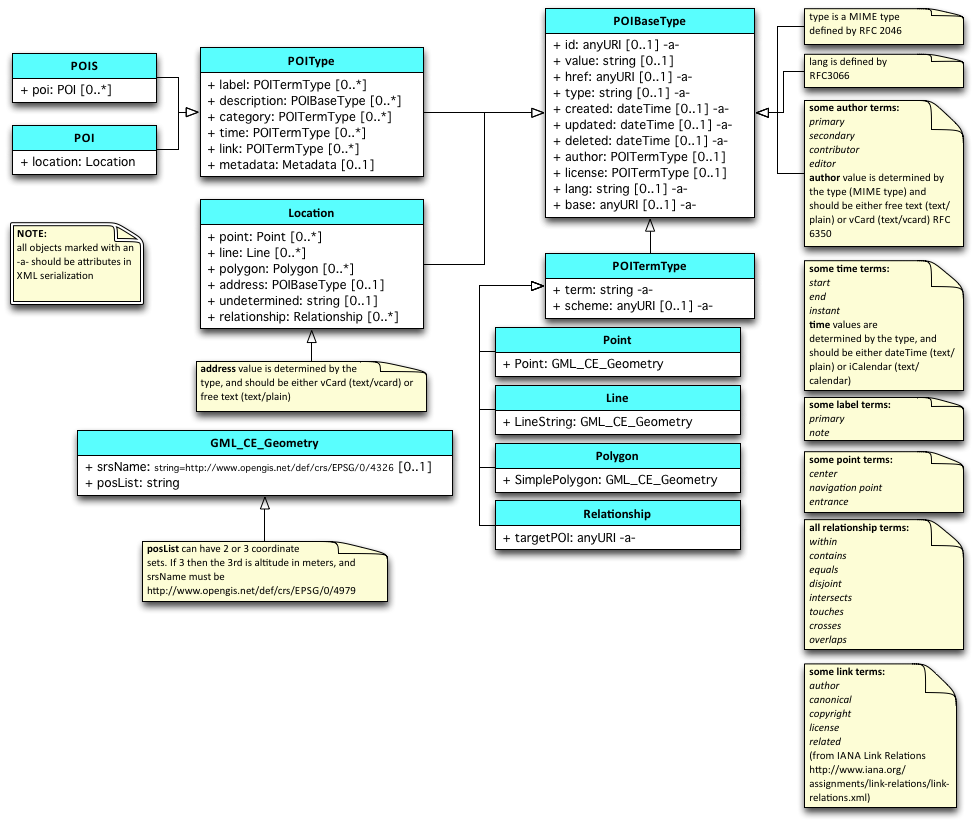
\includegraphics[scale=0.5]{W3c_poi_model.png}
	\caption{W3C UML Diagram POI Data Model}
	\label{fig:@=w3cDataModel}
\end{figure}
There is an apprehensible delamination in field of POI categories. It is difficult to find a standard which could be useful and well known for every data source. Fortunately there are standards defined by governments which describe categories in very detailed way and have endorsement by substantive position as countries governments possess. 
\subsection{NAICS}
\textit{\textbf{The North American Industry Classification System (NAICS)}} widely used in countries of North America. Developed by three organizations:  U.S. Economic Classification Policy Committee (ECPC), Statistics Canada, Mexico's Instituto Nacional de Estadistica y Geografia. It is mainly used by Federal agencies to collect data about bussiness entites for statistic purposes. It is successor of \textit{\textbf{Standard Industrial Classification (SIC)}}. NAICS classification is basing on codes which correspond to category description. Code can at most consist of six digits (the more digits included in code the more detailed category description is). Latest NAICS revision was issued in 2012. \cite{15} \cite{16}
\subsection{NACE}
\textit{\textbf{Statistical Classification of Economic Activities in the European Community (in French: Nomenclature statistique des activités économiques dans la Communauté européenne) - NACE}} system widely used in European Union. Similarly to NACE it is using combination of codes and category description. Code consists of letter and digits and creates special hierarchy of: sections, divisions, groups and classes. Section is marked by letter, division by two digits, groups and classes by one digit consecutively. Latest NACE revision (Rev.2) was issued in 2008 as a result of constantly developing and  newly appearing organizations especially in telecommunication business.\cite{17} \cite{18} Because java application which is purpose of this thesis was developed in Poland NACE categorization standard was chosen to apply in it. Obviously information included in NACE are definitely too much detailed to be applied for POI categorization system so only sections were taken into consideration. 

\section{Java library as categorization API}
\todo{cel api - zrodla danych, rezultat, metody processingu API = connection, classification, utilsy, czemu taki a nie inny podzial na pakiety - opis unit testow}
Main purpose of Java categorization API is to deliver an interface which would allow for convenient, correct and efficient results. API should be independent of data type which will be delivered. API responsibility is to enable functionalities (as this thesis states - categorization). To assure independence of data sources powerful mechanism of java interfaces can be used - such approach introduce level of abstraction and allow java library for easy communication with data sources. Java has very useful feature of importing and using libraries - when whole code is compiled to bytecode classes are bundled into resultant \textbf{\textit{.jar}} file - it can be immediately used in another java project by another programmer. Moreover, resultant java library project can be compiled with dependencies so programmer who will use library later will not have to bother about classes which were used during library development are were not part of Java API \cite{19}. This approach increases size of \textbf{\textit{.jar}} file but realease user from inconvenient dependencies downloading nad importing into project.    

\subsection{Packages organization}
API is divided into three packages: \textit{connection, classification} and \textit{utils}. Such packaging organization assures clear and concise representation of API functionalites and utilities. Functional packages are divided into simillar hierachy to interfaces and packages responsible for particular data source handling (see figure \ref{fig:@=packages_oragnization}). For purpose of this thesis these packages were named \textit{loadstone}. Obviously unit tests for corresponding executing classes are located into separate directory (according to maven directory structure \cite{20}) but are included in the same packages (for java it is counterpart of namespace).
\begin{figure}[h]
 	\centering
 	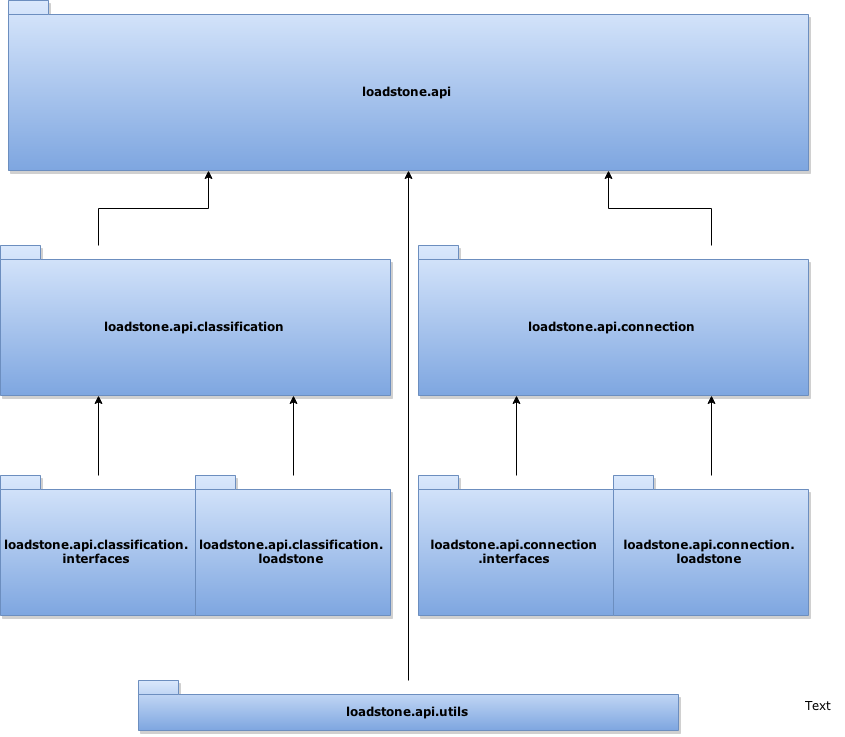
\includegraphics[scale=0.5]{loadstone_api_packages.png}
 	\caption{Loadstone API packages organization}
 	\label{fig:@=packages_oragnization}
\end{figure}
\subsection{Interface \newline loadstone.api.classification.interfaces.\newline AbstractResourcePreprocessing}
As mentioned before independence of input data is absolutely compulsory for API. To define preprocessing for each different kind of data source  AbstractResourcePreprocessing interface was defined. Classes which will be strictly delegated to preprocess particular source of data by implementation of this interface will be able to communicate with API and pass already preprocessed data for further classification methods.Interface also relies on model object data (DataModel) which is defined in another module of the project - \textbf{loadstone-model}. This assures for uniform and scalable solution for next data resources. AbstractResourcePreprocessing defines two methods which has to be implemented by data source dedicated classes to use categorization methods. Interface organization is depicted in the figure \ref{fig:@=AbstractResourcePreprocessing}:
\begin{figure}[h]
	\centering
	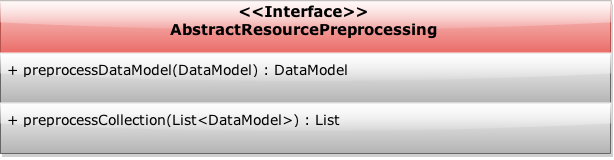
\includegraphics[scale=0.5]{AbstractResourcePreprocessing.png}
	\caption{AbstractResourcePreprocessing UML Diagram}
	\label{fig:@=AbstractResourcePreprocessing}
\end{figure}
\subsection{Interface \newline loadstone.api.classification.Classifier}
This interface is devoted for classes implementing classification functionalites. It imposes on classes to deliver data soure in appopriate way and return List. Main idea of this interface is to inform user that every data model object can be assigned to one or more classes. UML diagram on figure \ref{fig:@=classifier}
\begin{figure}[h]
	\centering
	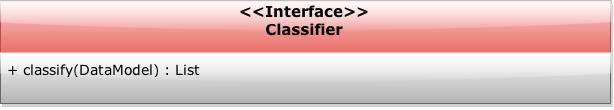
\includegraphics[scale=0.5]{classifier_interface.png}
	\caption{Interface Classifier UML Diagram}
	\label{fig:@=classifier}
\end{figure}
\subsection{Interface \newline loadstone.api.connection.interfaces.AbstractResourceConnection}
Interface to uniform the input point for data source to API. Each new data source should implement its own class for data gathering and return it in a way interface indicate it. Then data from any other resource (e.g. loadstone database, RESTful API) can be delivered for categorization functionalities. AbstractResourceConnection is simillar to AbstractResourcePreprocessing because of imposing data delivery in term of data model single object and its collection. Interface organization is depicted in the figure \ref{fig:@=connection}   
\begin{figure}[h]
	\centering
	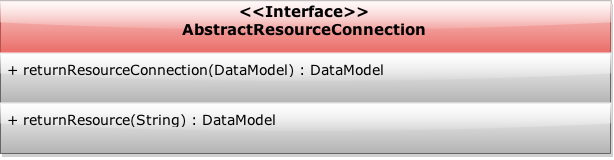
\includegraphics[scale=0.5]{Abstract_Resource_Connection_Interface.png}
	\caption{Interface AbstractResourceConnectionInterface UML Diagram}
	\label{fig:@=connection}
\end{figure}
Parameters for interface are respectively: List of Strings and String. Parameter types should be sufficient for particular data source invocation composition (e.g SQL statment). Using String type give user big flexibility if we are considering java as programming language.
\subsection{Class \newline loadstone.api.classification.loadstone.\newline LoadstonePreprocessing}
This class is deliberately delegated to preprocess data obtained from \textit{Loadstone} database. Using dedicated interface it assures final user about possibility of preprocesssing in easy to use and in the same time customized way. Class architecture is shown on \ref{fig:@=LoadstonePreprocessing}
\begin{figure}[h]
	\centering
	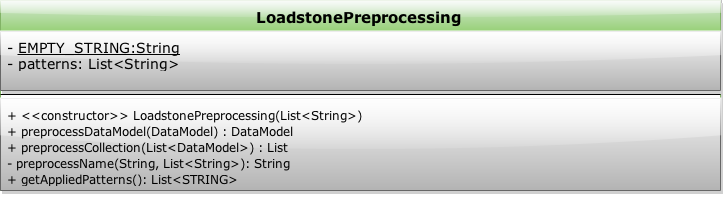
\includegraphics[scale=0.5]{LoadstonePreprocessing.png}
	\caption{LoadstonePreprocessing UML Diagram}
	\label{fig:@=LoadstonePreprocessing}
\end{figure}
Class organization is simple. For preprocessing functionality is responsible private method used in methods implementation of AbstractResourcePreprocessing interface. It simply process given input - rejects spaces (default behaviour) and patterns defined by user in constructor. Method is applied for single object DataModel or collection of such objects in corresponding interface methods.
\subsection{Class \newline loadstone.api.classification.loadstone.LoadstoneBOW}
\label{loadstone_bow}
This class is a feature for semi-supervised classification. It is basically a hashmap which values are sections of NACE categorization system and keys are strings which were the most frequenait occuring in loadstone database and assigned empirically to particular category. This class avails user to travers through map and check if category can be assigned immediately. 
\subsubsection{Bash script analyzeDB.sh}
\label{analyze_db}
Frequency for bag of words was prepared using bash shell script using awk tool which is great utility for text analysis \cite{21}. Script traverses through the loadstone database text file and counts occurrence of each word which exists in document. Algorithm can be expressed in following way:
\begin{algorithm}[h]
	\KwData{All words existing in loadstone database text file}
	\KwResult{Number of occurrences for each word}
	initalize array \textbf{words[]};
	\newline
	\ForEach{ \textit{word} in text file}
	{
		transform \textit{word} to lower case (avail disambiguation)
		\newline
		increase value by one for index \textit{word} in array \textbf{words[]} 
	}
	\ForEach{\textit{index-word} in \textbf{words[]}}{
		\Return word frequency:\textbf{words[\textit{index-word}]} for \textit{index-word} 	
	}
\caption{Analyzing frequency of words in database}\label{alg:analyze_freuency}
\end{algorithm}

Basing on Algorithm \ref{alg:analyze_freuency} it was possible to easily define those phrases which were most occuring and were significant or absolutely unncessary for text categorization. Obtaing list of words with their occurences in document there could be selected which can be used in BOW and which can be used for preprocessing as a hint.

\subsection{Class \newline loadstone.api.classification.NaiveClassifier}
\label{naive_classifier}
This class is implementing naive classification basing on descriptions from NACE\_Categories class using Classifier interface. It analyzes if data model name contains word which is included in particular category description. If data model name contains two or more words from distinct categories descriptions both of them are returned as possible categories to be assigned. This class is basing only on heuristic of NACE\_Categories descriptions so can be used for any data source but categorization correctness may differ significantly on data source.

\subsection{Class \newline loadstone.api.classification.loadstone.\newline LoadstoneSemiSupervisedClassifier}
Class which enables to classify POI using class LoadstoneBOW prepared previously. This class does not include descriptions from class NACE\_Categories. Only descriptions from LoadstoneBOW are taken into consideration. This class is implementing Classifier interface so it can be fluently used later in API.

\subsection{Class \newline loadstone.api.connection.loadstone.LoadstoneDatabase}
This class takes responsibility for gathering loadstone database. This class is implementing AbstractResourceConnection to get all possible entities from loadstone database. 
 
\subsubsection{LoadstoneDatabaseUpdater Singleton Design Pattern}
To modify data inside database loadstone.api.connection.loadstone.LoadstoneDatabaseUpdater should be used. It is using Singleton pattern to assure atomicity of operation on database. It defines static method \textit{getObjectModelSingleton()} returns static object on which user can work to modify data. Such approach allows for data correctness without bothering some other object is using database.  

\subsection{Class loadstone.api.utils.LoadstoneAPIUtils}
This class is just utility for user to construct appropriate SQL query to loadstone database. This utility only expect from user to input patterns which are supposed to be included during search for expected tuples in database. 

\subsection{Class loadstone.api.CategorizationAPI}
Class which can be enabled for final usage by user. It combines all methods of preprocessing, data source connection and classification methods. Should be used as input point for data considered to be classified and methods used for classification. Optionally user can add preprocessing method if step of this kind may be useful when POI classification is done.

\begin{figure}[h]
	\centering
	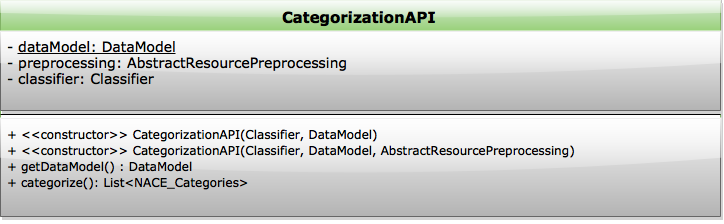
\includegraphics[scale=0.5]{CategorizationAPI.png}
	\caption{CategorizationAPI UML Diagram}
	\label{fig:@=CategorizationAPI}
\end{figure}

\addcontentsline{toc}{chapter}{Bibliography}
\bibliography{sources}{}
\bibliographystyle{alpha}

\end{document}
